\documentclass{CUP-JNL-DTM}%


%%%% Packages
\usepackage{graphicx}
\usepackage{multicol,multirow}
\usepackage{amsmath,amssymb,amsfonts}
\usepackage{mathrsfs}
\usepackage{amsthm}
\usepackage{rotating}
\usepackage{appendix}
% For JDM please remove the natbib package:
\usepackage[numbers]{natbib}
% And use biblatex-apa with a .bib file to format your references according to the APA7 style.
% \usepackage[natbib,style=apa]{biblatex}
% \addbibresource{your-refs.bib}
\usepackage{ifpdf}
\usepackage[T1]{fontenc}
\usepackage{newtxtext}
\usepackage{newtxmath}
\usepackage{textcomp}
\usepackage{xcolor}
\usepackage{lipsum}
\usepackage[colorlinks,allcolors=blue]{hyperref}

\newtheorem{theorem}{Theorem}[section]
\newtheorem{lemma}[theorem]{Lemma}
\theoremstyle{definition}
\newtheorem{remark}[theorem]{Remark}
\newtheorem{example}[theorem]{Example}
\numberwithin{equation}{section}


\jname{}
\articletype{}
%\artid{20}
\jyear{2024}
%\jvol{4}
%\jissue{1}
%\raggedbottom


\begin{document}

\begin{Frontmatter}

\title[Article Title]{Elaboraci\'on de la teor\'ia de expansi\'on de Mayer}

% There is no need to include ORCID IDs in your .pdf; this information is captured by the submission portal when a manuscript is submitted. 
\author[1]{Jos\'e David Ochoa Flores}

\authormark{Author Name1 \textit{et al}.}

\address[1]{\orgdiv{Maestr\'ia de F\'isica}, \orgname{Universidad San Francisco de Quito}, \orgaddress{\city{Quito}, \country{Ecuador}}}


\authormark{Author Name1 et al.}

\keywords{keyword1, keyword2, keyword3, keyword4}


\abstract{Abstracts should be 250 words. It must be able to stand alone and so cannot contain citations to the paper's references, equations, etc. An abstract must consist of a single paragraph and be concise. Because of online formatting, abstracts must appear as plain as possible.}

\end{Frontmatter}

% Some math journals (FLO) require a table of contents. Comment out this line if no ToC is needed.
\localtableofcontents

\section[Seccion 1]{Seccion 1}
Seccion 1 sdlfjasdfljasdlfjhasdlfjahsldfjasldfjasdljfasldfj

\subsection{Subseccion 1}

Subseccion 1 jlkahsfjkhsadlfjkhasldfasdf

\subsubsection{Sub sub seccion 1}

Sub sub seccion 1jasdlfjhasldfjkhasldfjkasdf

\paragraph{This is a D head this is a D head this is a D head this is a D head}

palabras palabras

\section[Seccion 2]{Seccion 2}
palabras palabraspalabras palabraspalabras palabraspalabras palabraspalabras palabras
\subsection{Subseccion 2.1}
palabras palabraspalabras palabraspalabras palabraspalabras palabraspalabras palabras
\subsubsection{sub subseccion 2.1.1}
palabras palabraspalabras palabraspalabras palabraspalabras palabraspalabras palabras

hola \footnote{This is sample for footnote this is sample for footnote this is sample for footnote  this is sample for footnote this is sample for footnote.}

\section{Equations}

Equations in \LaTeX{} can either be inline or on-a-line by itself. For
inline equations use the \verb+$...$+ commands. Eg: The equation
$H\psi = E \psi$ is written via the command $H \psi = E \psi$.

For on-a-line by itself equations (with auto generated equation numbers)
one can use the equation or eqnarray environments \textit{D}.
\begin{equation}
\mathcal{L} = i {\psi} \gamma^\mu D_\mu \psi
    - \frac{1}{4} F_{\mu\nu}^a F^{a\mu\nu} - m {\psi} \psi
\label{eq1}
\end{equation}

\begin{equation}
    B^{+} \rightarrow K^{+}H' (\rightarrow \mu^{+} \mu^{-})
\end{equation}
where,
\begin{align}
D_\mu &=  \partial_\mu - ig \frac{\lambda^a}{2} A^a_\mu
\nonumber \\
F^a_{\mu\nu} &= \partial_\mu A^a_\nu - \partial_\nu A^a_\mu
    + g f^{abc} A^b_\mu A^a_\nu
\label{eq2}
\end{align}
Notice the use of \verb+\nonumber+ in the align environment at the end
of each line, except the last, so as not to produce equation numbers on
lines where no equation numbers are required. The \verb+\label{}+ command
should only be used at the last line of an align environment where
\verb+\nonumber+ is not used.
\begin{equation}
Y_\infty = \left( \frac{m}{\textrm{GeV}} \right)^{-3}
    \left[ 1 + \frac{3 \ln(m/\textrm{GeV})}{15}
    + \frac{\ln(c_2/5)}{15} \right]
\end{equation}
The class file also supports the use of \verb+\mathbb{}+, \verb+\mathscr{}+ and
\verb+\mathcal{}+ commands. As such \verb+\mathbb{R}+, \verb+\mathscr{R}+
and \verb+\mathcal{R}+ produces $\mathbb{R}$, $\mathscr{R}$ and $\mathcal{R}$
respectively.

\section{Figures}

As per the \LaTeX\ standards eps images in \verb!latex! and pdf/jpg/png images in
\verb!pdflatex! should be used. This is one of the major differences between \verb!latex!
and \verb!pdflatex!. The images should be single page documents. The command for inserting images
for latex and pdflatex can be generalized. The package that should be used
is the graphicx package.

\begin{figure}[t]%
\FIG{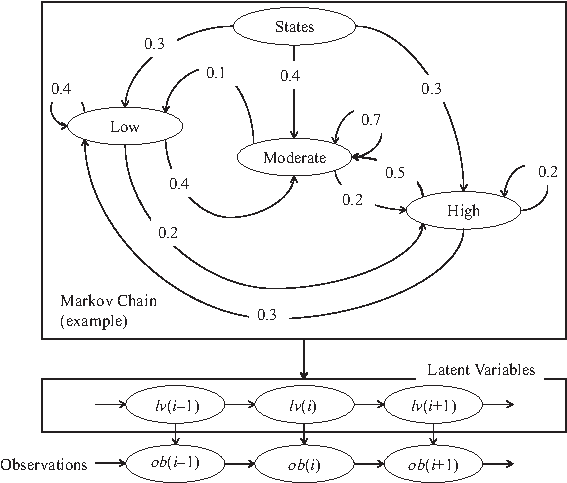
\includegraphics[width=0.9\textwidth]{Fig}}
{\caption{This is a widefig. This is an example of long caption this is an example of long caption  this is an example of long caption this is an example of long caption}
\label{fig1}}
\end{figure}



\section{Tables}

Tables can be inserted via the normal table and tabular environment. To put
footnotes inside tables one has to use the additional ``fntable" environment
enclosing the tabular environment. The footnote appears just below the table
itself.

\begin{table}[t]
\tabcolsep=0pt%
\TBL{\caption{Tables which are too long to fit,
should be written using the ``table*'' environment as~shown~here\label{tab2}}}
{\begin{fntable}
\begin{tabular*}{\textwidth}{@{\extracolsep{\fill}}lcccccc@{}}\toprule%
 & \multicolumn{3}{@{}c@{}}{\TCH{Element 1}}& \multicolumn{3}{@{}c@{}}{\TCH{Element 2\smash{\footnotemark[1]}}}
 \\\cmidrule{2-4}\cmidrule{5-7}%
\TCH{Projectile} & \TCH{Energy} & \TCH{$\sigma_{\mathit{calc}}$} & \TCH{$\sigma_{\mathit{expt}}$} &
\TCH{Energy} & \TCH{$\sigma_{\mathit{calc}}$} & \TCH{$\sigma_{\mathit{expt}}$} \\\midrule
\TCH{Element 3}&990 A &1168 &$1547\pm12$ &780 A &1166 &$1239\pm100$\\
{\TCH{Element 4}}&500 A &961 &$\hphantom{0}922\pm10$ &900 A &1268 &$1092\pm40\hphantom{0}$\\
\botrule
\end{tabular*}%
\footnotetext[]{{Note:} This is an example of table footnote this is an example of table footnote this is an example of table footnote this is an example of~table footnote this is an example of table footnote}
\footnotetext[1]{This is an example of table footnote}%
\end{fntable}}
\end{table}



\section{Cross referencing}

Environments such as figure, table, equation, align can have a label
declared via the \verb+\label{#label}+ command. For figures and table
environments one should use the \verb+\label{}+ command inside or just
below the \verb+\caption{}+ command.  One can then use the
\verb+\ref{#label}+ command to cross-reference them. As an example, consider
the label declared for Figure \ref{fig1} which is
\verb+\label{fig1}+. To cross-reference it, use the command
\verb+ Figure \ref{fig1}+, for which it comes up as
``Figure \ref{fig1}''.
The reference citations should used as per the ``natbib'' packages. Some sample citations:  \cite{bib1,bib2,bib3,bib4,bib5}.




\section{Conclusion}

Some Conclusions here.



\begin{Backmatter}
% For JDM please remove this \begin{thebibliography}...\end{thebibliography} list.
% Use biblatex-apa (see instructions in preamble) instead, and write \printbibliography here to print the reference list in APA7 style.
\begin{thebibliography}{}
\bibitem[Ananin A. and Mironov A.(2000)]{bib1}
\textbf{Ananin A. and Mironov A.} (2000) The moduli space of $2$-dimensional algebras, \textit{Comm. Algebra} \textit{28}(9),  {4481}--{4488}.

\bibitem[Bai C. and Meng D.(2001)]{bib2}
\textbf{Bai C. and Meng D.} (2001) The classification of Novikov algebras in low dimension,  \textit{J. Phys. A: Math. Gen.} \textit{34}, {1581}--{1594}.

\bibitem[Ca\~{n}ete E. and Khudoyberdiyev A.(2013)]{bib3}
\textbf{Ca\~{n}ete E. and Khudoyberdiyev A.} (2013) The classification of $4$-dimensional Leibniz algebras,  \textit{Linear Algebra and its Applications}  \textit{439}(1), {273}--{288}.

\bibitem[Goze M. and Remm E.(2011)]{bib4}
\textbf{Goze M. and Remm E.} (2011)  $2$-dimensional algebras,  \textit{Afr. J. Math. Phys.} \textit{10}(1),  {81}--{91}.

\bibitem[Petersson H.(2000)]{bib5}
\textbf{Petersson H.} (2000) The classification of two-dimensional nonassociative algebras,  \textit{Results Math} \textit{37}, no. 1-2,  {120}--{154}.


\end{thebibliography}

\end{Backmatter}

\end{document}
